\documentclass[12pt]{article}

\usepackage[utf8]{inputenc}
\usepackage{datetime}
\usepackage{amsthm}
\usepackage{amsmath}
\usepackage{amssymb}
\usepackage{enumitem}
\usepackage[USenglish]{babel}
\usepackage{matlab-prettifier}
\usepackage{graphicx}
\usepackage[makeroom]{cancel}
\usepackage{afterpage}
\usepackage{capt-of}

\DeclareMathOperator*{\argmin}{arg\,min}
\DeclareMathOperator*{\argmax}{arg\,max}

\newcommand\independent{\protect\mathpalette{\protect\independenT}{\perp}}
\def\independenT#1#2{\mathrel{\rlap{$#1#2$}\mkern2mu{#1#2}}}

\newtheoremstyle{colon}{\topsep}{\topsep}{}{}{\bfseries}{:}{ }{}
\theoremstyle{colon}
\newtheorem{exercise}{Exercise}
\newtheorem*{answer}{Answer}

\title{ORFE 525: Statistical Learning and \\ Nonparametric Estimation \\ Homework 3}
\author{Zachary Hervieux-Moore}

\newdate{date}{06}{04}{2017}
\date{\displaydate{date}}

\begin{document}

\maketitle

\clearpage

\begin{exercise}
  The goal is to build a classifier of images, the two classes being: having humans or not. The two provided datasets \texttt{POS} and \texttt{NEG} have photos with and without upright humans respectively.

  \begin{enumerate}[label=\arabic*)]
    \item Preprocessing the data
      \begin{enumerate}[label=\alph*)]
        \item Randomly pick out one image in \texttt{NEG} and one in \texttt{POS}. For each of the two images, implement each step below to vectorize and extract useful information. We provide functions that will be used in the following steps in a R-script \texttt{functions.r}. Please CAREFULLY read the appendix for the detailed introductions of these functions.
          \begin{enumerate}[label=\arabic*)]
            \item Download and install the package \texttt{png}, and use the function \texttt{readPNG} to load photos.
            \item Use the function \texttt{rgb2gray} to transform the original photos to the black and white version.
            \item Since photos in \texttt{NEG} have bigger sizes than those in \texttt{POS} we need to crop them to keep consistency in dimensions. So for all photos \texttt{NEG}, use the function \texttt{crop.r} to randomly crop a $160 \times 96$ picture from the original one.
            \item Use the function \texttt{grad} to obtain the gradient field of the center $128 \times 64$ part of the grayscale matrix.
            \item Use the function \texttt{hog} (Histograms of Oriented Gradient) to extract a feature vector from the gradient field obtained in the previous step. Partition the height and width into 4 partitions each. Partition the angle into 6 intervals. (Your feature vector should then have $4 \times 4 \times 6 = 96$ components). Please see the appendix for parameter configuration of this function.
          \end{enumerate}
          For each of the two images, provide a picture showing each step above, i.e., the original picture $\rightarrow$ the black and white picture $\rightarrow$ the cropped picture (for $\texttt{NEG}$) $\rightarrow$ the gradient field $\rightarrow$ the feature vector. For the feature vector, report its first six components.

        \item Now, apply the above procedure to obtain feature vectors for each image in the dataset. Concatenate the feature vectors together into rows of a dataframe. Add an additional column indicatin whether each row is in \texttt{POS} or \texttt{NEG}. This will be the dataset you will use in Question 1.2.
      \end{enumerate}

    \item Detect the upright man

      In this question, we will apply both SVM and Logistic regression to train the model and compare their performance.
      \begin{enumerate}[label=\arabic*)]
        \item Download the package \texttt{kernlab}. Use the functions \texttt{ksvm} to train the model. Given the tuning parameter $C$ and the number of folds $k$, \texttt{ksvm} can return the cross-validation error. Examine how the cross-validation error changes as we tune $C$ in the range of $[0.0001, 100]$ as follows:

          \begin{itemize}
            \item Construct a sequence of 100 values of $C$ such that $\ln (C)$ is an arithmetic series with $\ln (10^{-4})$ as the minimum and $\ln (10^2)$ as the maximum.
            \item Plot out the misclassification error against $\ln(C)$.
            \item Find out the optimal $C$ in the sequence that yields the lowest misclassification error.
          \end{itemize}
        \item Use the function \texttt{glmnet} to train the model via logistic regression and plot out the regularization path. More importantly, use the function \texttt{cv.glmnet} to do the cross-validation with the option \texttt{type.measure=``class''}. Plot the results.
        \item Compare the lowest cross-validation error of SVM and logistic regression. Do they differ significantly?
      \end{enumerate}
  \end{enumerate}
\end{exercise}

\begin{answer}
  \leavevmode
  \begin{enumerate}[label=\arabic*)]
    \item All the code used is in the appendix below.
      \begin{enumerate}[label=\alph*)]
        \item I used picture 193 from \texttt{POS} and 60 from \texttt{NEG}. Figures 1 and 2 show their preprocessing. Figure 3 shows the gradient for \texttt{NEG} 60. Finally, the first 6 entries in the feature vector are:
          \begin{gather*}
            \text{feature}_{POS} = [0.1816, 0.1309, 0.1484, 0.1660, 0.1875, 0.1855, \mathellipsis] \\
            \text{feature}_{NEG} = [0.1211, 0.1074, 0.0566, 0.0020, 0.1387, 0.0117, \mathellipsis]
          \end{gather*}

          \begin{center}
            
\includegraphics[height=4cm]{193.png}
            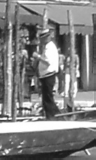
\includegraphics[height=4cm]{grey_193.png}
            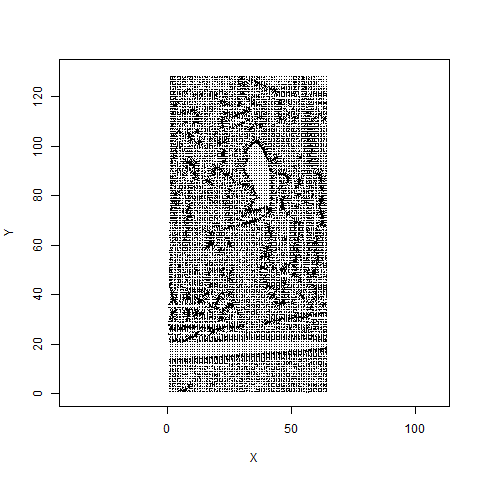
\includegraphics[height=4cm]{grad_193.png}
            \captionof{figure}{Preprocessing of \texttt{POS} 193}
          \end{center}

          \begin{center}
            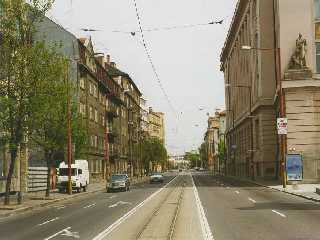
\includegraphics[height=3cm]{60.png}
            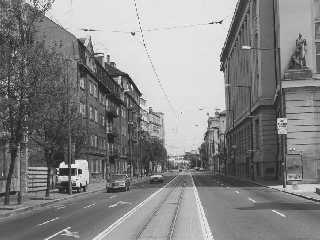
\includegraphics[height=3cm]{grey_60.png}
            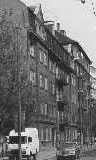
\includegraphics[height=3cm]{crop_60.png}
            \captionof{figure}{Preprocessing of \texttt{NEG} 60}
          \end{center}

          \begin{center}
            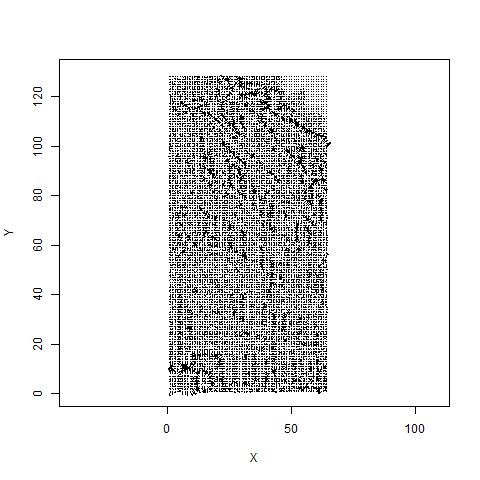
\includegraphics[width=0.5\textwidth]{grad_60.png}
            \captionof{figure}{Gradient \texttt{NEG} 60}
          \end{center}

        \item Code in appendix
      \end{enumerate}

    \item
      \begin{enumerate}[label=\arabic*)]
        \item The cross-validation error as $\ln(C)$ changes is in Figure 4. The optimal $C$ is 86.97.
          \begin{center}
            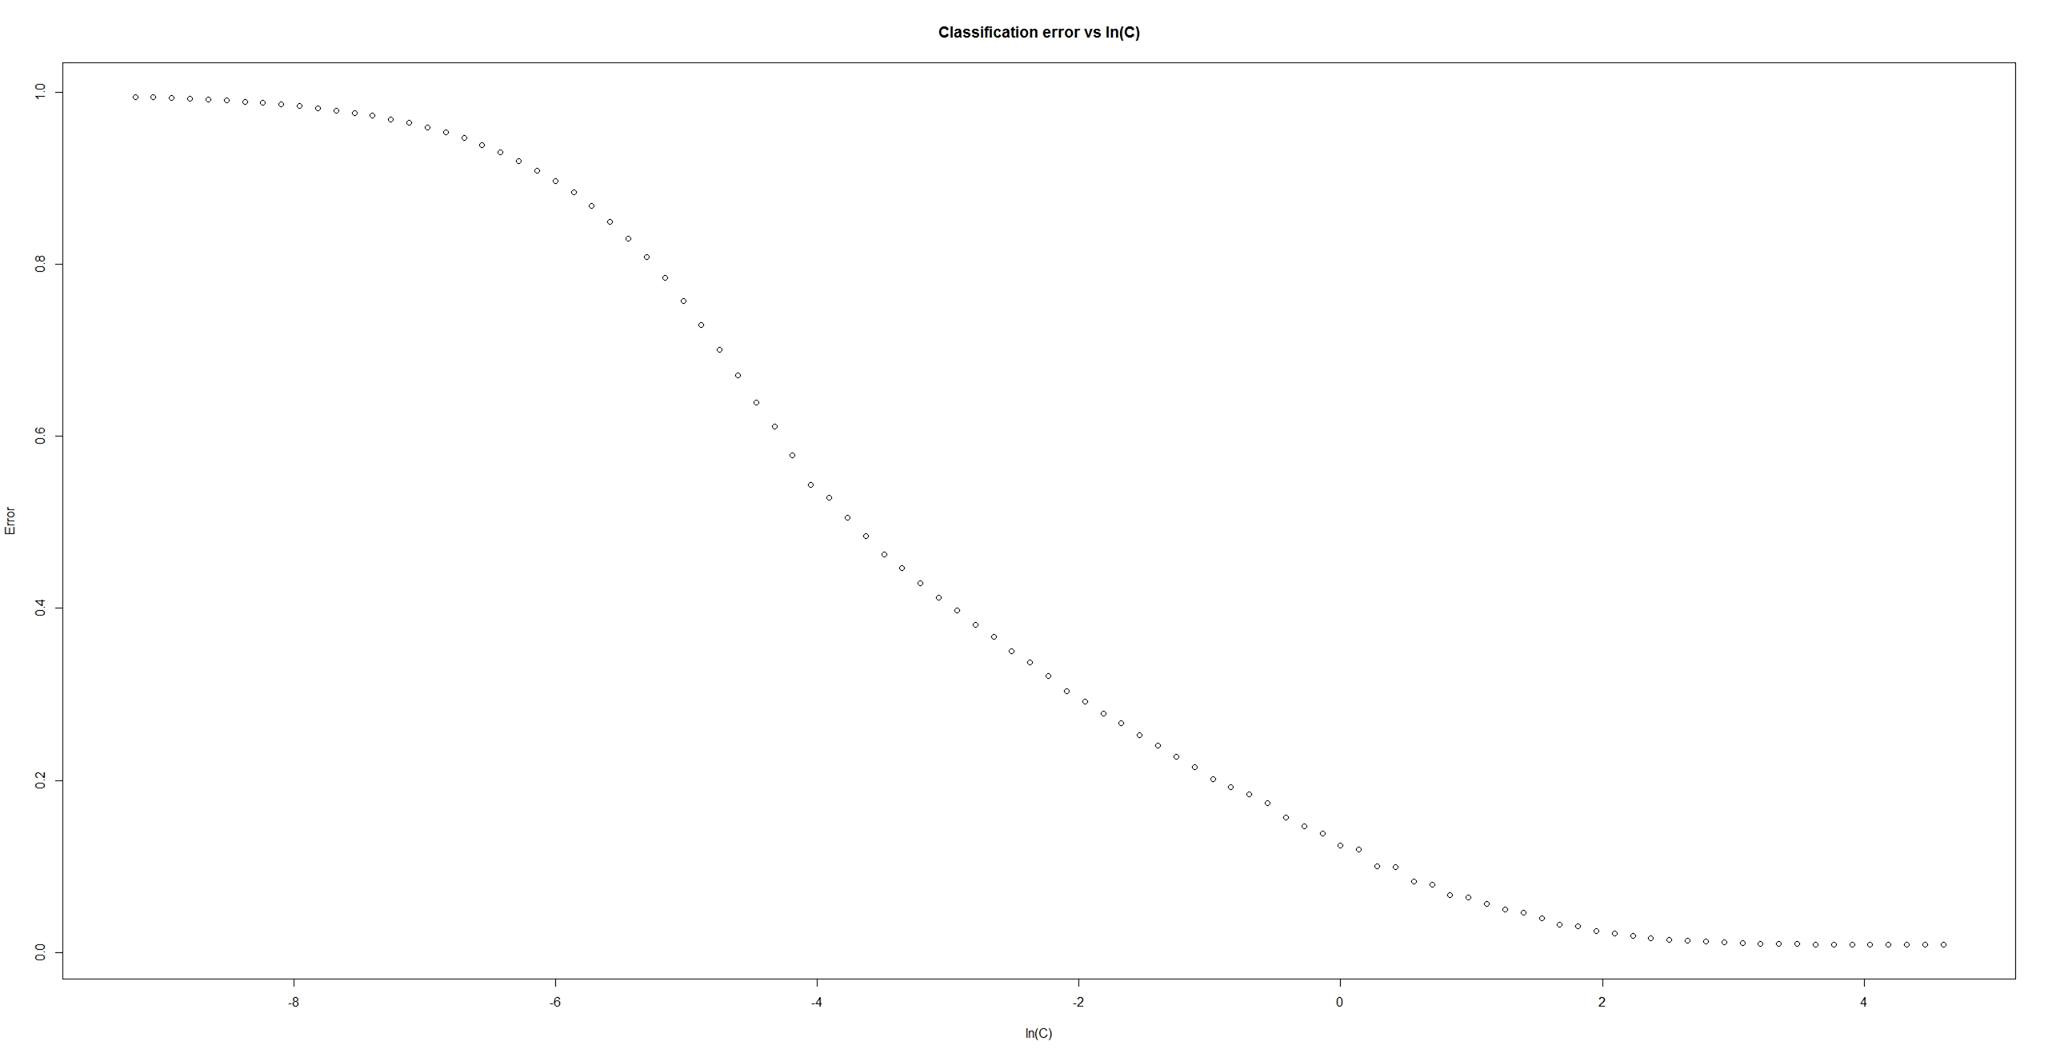
\includegraphics[width=0.8\textwidth]{svm_error.jpg}
            \captionof{figure}{Cross-Validation error vs $\ln(C)$}
          \end{center}

        \item The regularization paths are in Figure 5 and misclassification error is in Figure 6
          \begin{center}
            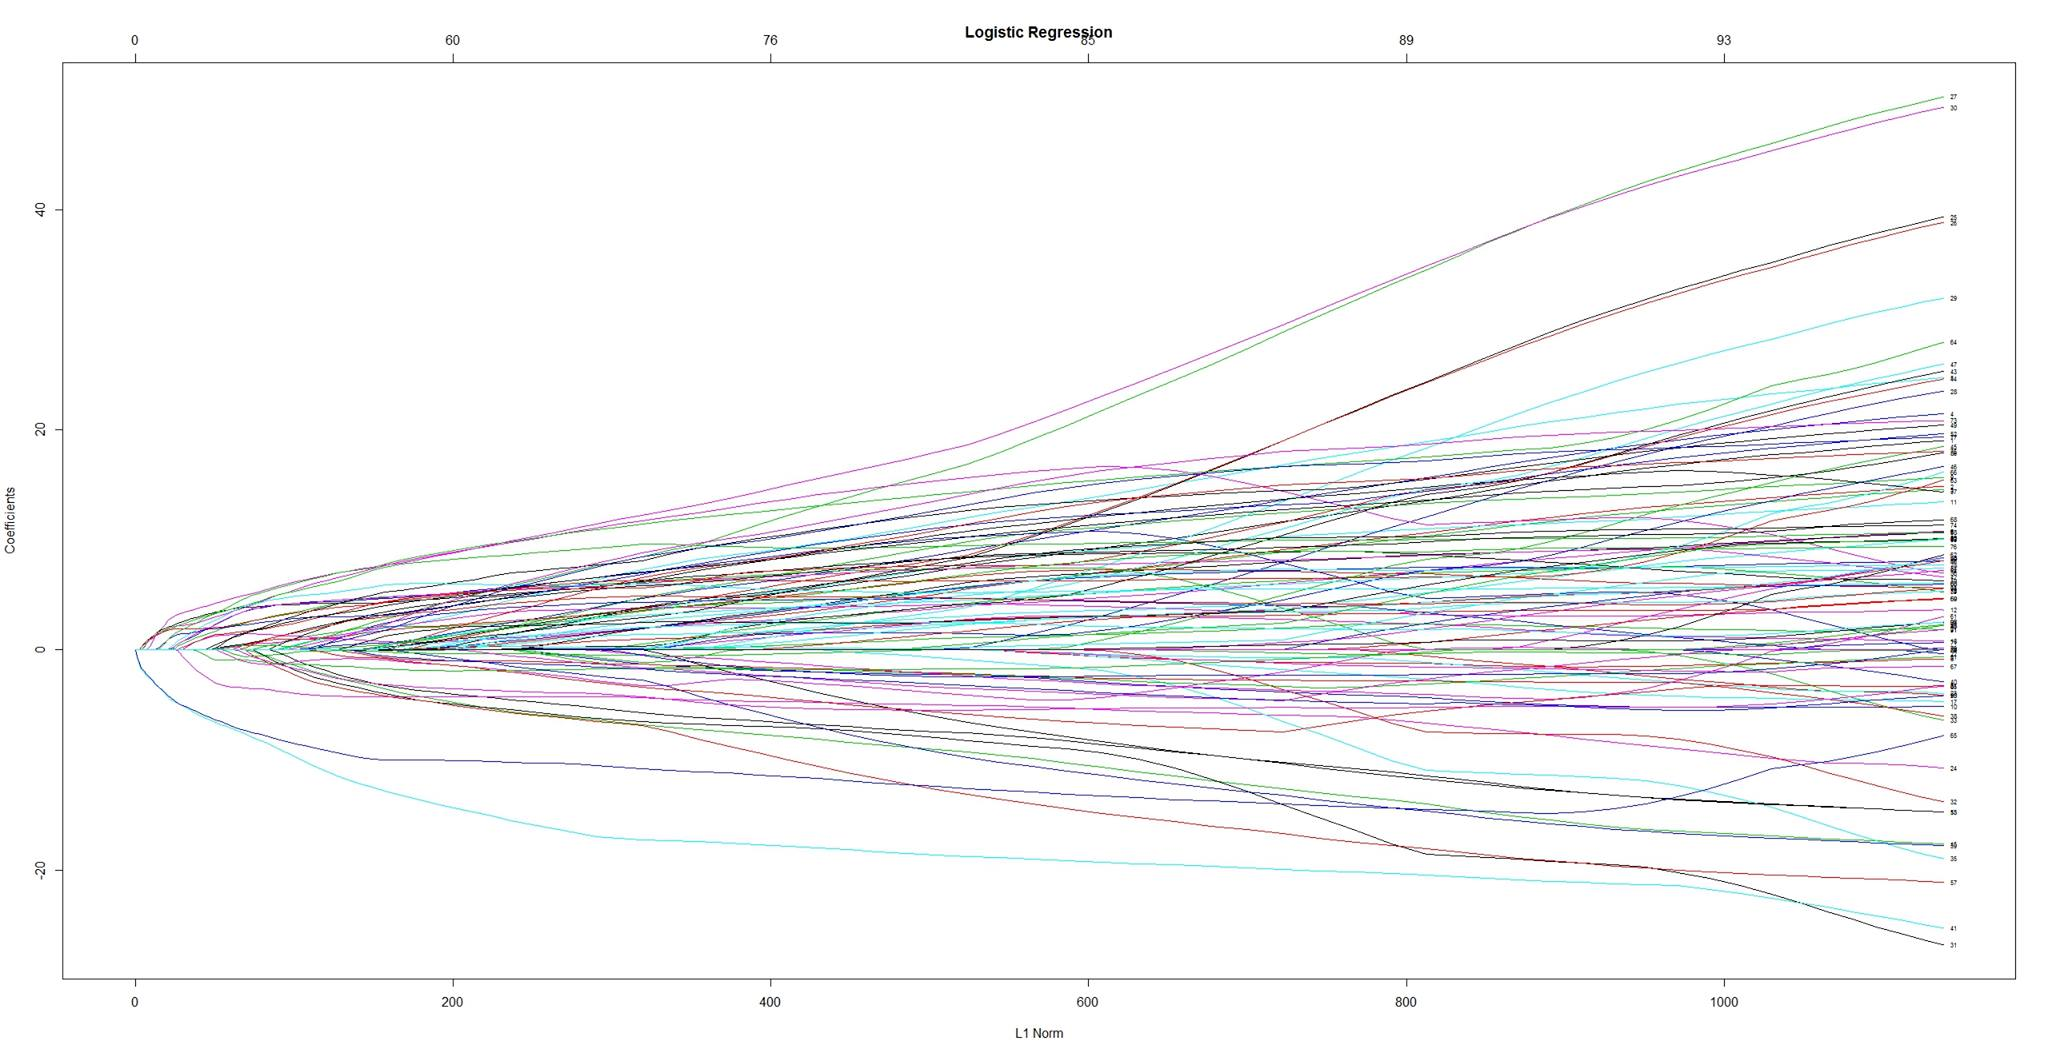
\includegraphics[width=0.8\textwidth]{glm_paths.jpg}
            \captionof{figure}{Regularization Paths for Logistic Regression}
          \end{center}

          \begin{center}
            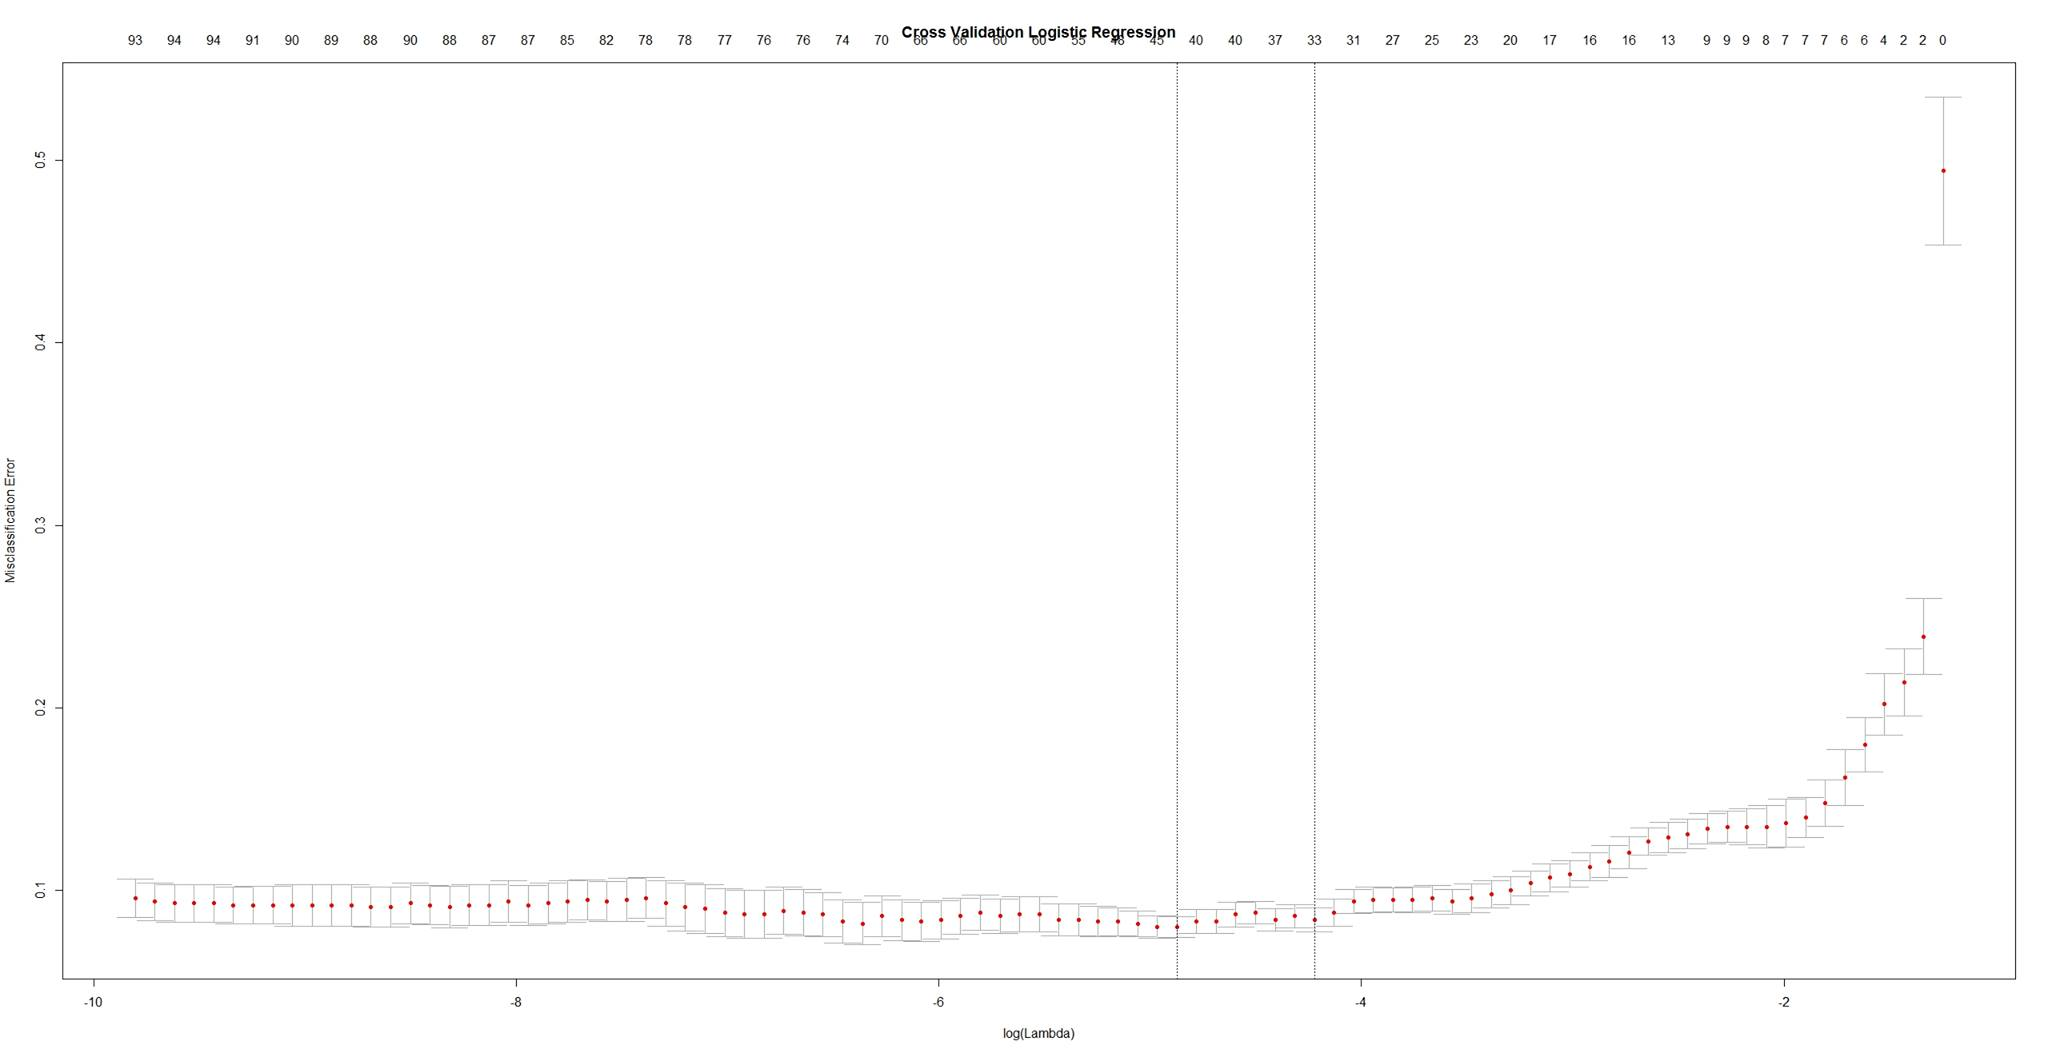
\includegraphics[width=0.8\textwidth]{cv_glm.jpg}
            \captionof{figure}{Misclassfication vs $\log(\lambda)$}
          \end{center}

        \item The minimum cross-validation error for logistic regression is 0.083 while the minimum misclassification for SVM is 0.0088. This is a difference of an order of magnitude which is very significant.
      \end{enumerate}
  \end{enumerate}

  \textbf{Code Appendix}

  \begin{lstlisting}[language=R, basicstyle=\scriptsize, breaklines=true]
    # Part 1.1
    library(png)
    source('./functions.r')

    ## Need to create folders ./grey_pos and ./grey_neg
    ## and folders ./grad_pos and ./grad_neg

    files <- list.files(path="./pos", pattern="*.png", full.names=T, recursive=FALSE)
    lapply(files, function(x) {
      name <- basename(x)
      p <- readPNG(x)
      p <- rgb2gray(p)
      writePNG(p, target = paste("./grey_pos/", name, sep=""))
      png(paste("./grad_pos/", name, sep=""))
      g <- grad(p, 128, 64, TRUE)
      dev.off()
    })

    files <- list.files(path="./neg", pattern="*.png", full.names=T, recursive=FALSE)
    lapply(files, function(x) {
      name <- basename(x)
      n <- readPNG(x)
      n <- rgb2gray(n)
      n <- crop.r(n,160,96)
      writePNG(n, target = paste("./grey_neg/", name, sep=""))
      png(paste("./grad_neg/", name, sep=""))
      g <- grad(n, 128, 64, TRUE)
      dev.off()
    })

    # Part 1.1a
    ## Using pos=193, neg=60, all images saved from the above

    data.pos <- readPNG("./pos/193.png")
    data.pos <- rgb2gray(data.pos)
    data.pos.grad  <- grad(data.pos, 128, 64, FALSE)
    data.pos.feature <- hog(data.pos.grad$xgrad, data.pos.grad$ygrad, 4, 4, 6)
    data.pos.feature[1:6]

    data.neg <- readPNG("./neg/60.png")
    data.neg <- rgb2gray(data.neg)
    writePNG(data.neg, target = "./cropped_60.png")
    data.neg <- crop.r(data.neg,160,96)
    data.neg.grad  <- grad(data.neg, 128, 64, FALSE)
    data.neg.feature <- hog(data.neg.grad$xgrad, data.neg.grad$ygrad, 4, 4, 6)
    data.neg.feature[1:6]

    # Part 1.1b

    data.df <- data.frame(matrix(NA, ncol=97, nrow=0))

    files <- list.files(path="./pos", pattern="*.png", full.names=T, recursive=FALSE)
    lapply(files, function(x) {
      name <- basename(x)
      p <- readPNG(x)
      p <- rgb2gray(p)
      g <- grad(p, 128, 64, FALSE)
      h <- hog(g$xgrad, g$ygrad, 4, 4, 6)
      # 1 because POS
      data.df <<- rbind(data.df, c(h,1))
    })

    files <- list.files(path="./neg", pattern="*.png", full.names=T, recursive=FALSE)
    lapply(files, function(x) {
      name <- basename(x)
      n <- readPNG(x)
      n <- rgb2gray(n)
      g <- grad(n, 128, 64, FALSE)
      h <- hog(g$xgrad, g$ygrad, 4, 4, 6)
      # 0 because NEG
      data.df <<- rbind(data.df, c(h,0))
    })


    names(data.df) <- c(paste("hog_", 1:96, sep=""),"POS")

    # Part 1.2

    library(kernlab)

    ln_C <- seq(log(0.0001), log(100), length.out = 100)
    C = exp(ln_C)

    svm.error <- sapply(C, function(x){
      ksvm(POS ~ ., data=data.df, C=x, cross=5)
    }@error)

    ## Plot error vs ln(C)

    dev.new()
    plot(ln_C, svm.error, main="Classification error vs ln(C)", xlab="ln(C)", ylab="Error")

    ## Optimal C

    C.optimal <- C[which.min(svm.error)]
    print("Optimal C value for SVM:")
    C.optimal
    print("CV error of SVM for optimal C:")
    min(svm.error)

    ## glmnet
    library(glmnet)

    x = data.matrix(data.df[,1:96])
    y = data.matrix(data.df[,97])

    model.glm <- glmnet(x, y, family="binomial")
    model.glm.cv <- cv.glmnet(x, y, family="binomial", type.measure="class")

    ## Plots

    dev.new()
    plot(model.glm, label=TRUE)
    title(main="Logistic Regression")

    dev.new()
    plot(model.glm.cv)
    title(main="Cross Validation Logistic Regression")

    ## Lowest CV error

    print("CV error of SVM for optimal lambda:")
    min(model.glm.cv$cvm)
  \end{lstlisting}
\end{answer}

\clearpage

\begin{exercise}
  Suppose that $\mathbb{P}(Y=1) = 1/3$, $\mathbb{P}(Y=-1) = 2/3$ and $X|Y = -1 \sim $ Uniform(-10,5) and $X|Y = 1 \sim $ Uniform(-5,10)
  \begin{enumerate}[label=\alph*)]
    \item Find an expression for the Bayes classifier and find an expression for the Bayes risk.
    \item Consider the classifier $h(x) = \text{sign}(\alpha + \beta x^2)$ where $\alpha, \beta \in \mathbb{R}$. Find at least one classifer $(\alpha^*, \beta^*)$ which minimizes the risk and what is its risk?
    \item Compute the hinge risk $R_\phi (\beta) = \mathbb{E}[(1-Y \beta X)_+]$ where \\ $(x)_+ = \max \{x, 0\}$.
  \end{enumerate}
\end{exercise}

\begin{answer}
  \leavevmode
  \begin{enumerate}[label=\alph*)]
    \item We have by Bayes rule that $p(y|x) = \frac{p(x|y)p(y)}{p(x)}$. In this case
      \begin{align*}
        \mathbb{P}(Y = 1 | X) &= \frac{\frac{1}{15} 1_{[-5,10]} \cdot \frac{1}{3}}{\mathbb{P}(X | Y=1)\mathbb{P}(Y=1)+\mathbb{P}(X | Y=-1)\mathbb{P}(Y=-1)} \\
        &= \frac{\frac{1}{45}1_{[-5,10]}}{\frac{1}{45}1_{[-5,10]} + \frac{2}{45}1_{[-10,5]}} \\
        &= \frac{1_{[-5,10]}}{1_{[-5,10]} + 2 \cdot 1_{[-10,5]}}
      \end{align*}
      Similarly,
      \begin{gather*}
        \mathbb{P}(Y = -1 | X) = \frac{2 \cdot 1_{[-10,5]}}{1_{[-5,10]} + 2 \cdot 1_{[-10,5]}}
      \end{gather*}
      Thus, the classifier is
      \begin{gather*}
        h^*(x) := \argmax_{Y \in \{-1,1\}} \mathbb{P}(Y|X=x) = 1_{[5,10]} - 1_{[-10,5]}
      \end{gather*}
      The Bayes risk is then
      \begin{align*}
        \mathbb{E}[1_{h^*(x) \neq Y}] &= \mathbb{P}(Y = 1, h(X) = -1) + \mathbb{P}(Y = -1, h(X) = 1) \\
        &= \mathbb{P}(h(X) = -1 | Y = 1)\mathbb{P}(Y = 1)\\
        &\quad + \mathbb{P}(h(X) = 1 | Y = -1)\mathbb{P}(Y = -1) \\
        &= \mathbb{P}(X \in [-5,5] | Y = 1)\mathbb{P}(Y = 1) + 0 \\
        &= \frac{2}{3} \cdot \frac{1}{3} = \frac{2}{9}
      \end{align*}

    \item If $h(x) = \text{sign}(\alpha + \beta x^2)$. The risk then becomes
      \begin{align*}
        R(h) = \mathbb{E}[1_{h^*(x) \neq Y}] &= \mathbb{P}(h(X) = -1 | Y = 1)\mathbb{P}(Y = 1)\\
        &\quad + \mathbb{P}(h(X) = 1 | Y = -1)\mathbb{P}(Y = -1) \\
        &= \frac{1}{3} \mathbb{P}(\alpha + \beta x^2 < 0 | Y = 1) + \frac{2}{3} \mathbb{P}(\alpha + \beta x^2 \geq 0 | Y = -1) \\
      \end{align*}
      From here, it is clear that if $\alpha \geq 0$ and $\beta \geq 0$ then $R(h) = 2/3$. If $\alpha < 0$ and $\beta \leq 0$ then $R(h) = 1/3$. Now consider the case when $\alpha < 0$ and $\beta \geq 0$. Then we have
      \begin{gather*}
        R(h) = \frac{1}{3} \mathbb{P}(X < \sqrt{-\frac{\alpha}{\beta}} | Y = 1) + \frac{2}{3} \mathbb{P}(X \geq \sqrt{-\frac{\alpha}{\beta}} | Y = -1)
      \end{gather*}
      Then suppose that $\sqrt{-\frac{\alpha}{\beta}} = c$, then we have
      \begin{gather*}
        R(h) = \frac{1}{45}\begin{cases}
          15 & \text{ if } c \geq 10 \\
          25 - c & \text{ if } 5 < c < 10 \\
          30 - 2c \text{ if } 0 \leq c \leq 5
        \end{cases}
      \end{gather*}
      Likewise, for the case $\alpha \geq 0$ and $\beta < 0$ we have
      \begin{gather*}
        R(h) = \frac{1}{45}\begin{cases}
          30 & \text{ if } c \geq 10 \\
          20 + c & \text{ if } 5 < c < 10 \\
          15 + 2c \text{ if } 0 \leq c \leq 5
        \end{cases}
      \end{gather*}
      One minimizer of this is $(\alpha^*, \beta^*) = (-1,0)$ which yields a risk of 1/3.

    \item When $\beta = 0$, we have $R_\phi(0) = 1$. For $\beta > 0$, we use the law of total expectation
      \begin{align*}
        R_\phi(\beta) &= \mathbb{E}[(1-Y \beta X)_+] \\
        &= \mathbb{E}[(1-\beta X)_+] \mathbb{P}(Y=1) + \mathbb{E}[(1+\beta X)_+] \mathbb{P}(Y=-1) \\
        &= \frac{1}{3} \int_{-5}^10 \frac{1}{15} (1 - \beta x)_+ dx + \frac{2}{3} \int_{-10}^5 \frac{1}{15} (1 + \beta x)_+ dx
      \end{align*}
      Change of variable $x' = \beta x$
      \begin{align*}
        &= \frac{1}{45 \beta} \int_{-5 \beta}^{10 \beta} (1 - x)_+ dx + \frac{2}{45 \beta} \int_{-10 \beta}^{5 \beta} (1 + x)_+ dx \\
        &= \frac{1}{45 \beta} \int_{-5 \beta}^{\min(10 \beta, 1)} (1 - x)_+ dx + \frac{2}{45 \beta} \int_{\max(-10 \beta,-1)}^{5 \beta} (1 + x)_+ dx \\
        &= \frac{1}{45 \beta} ( \min(10 \beta, 1) + 5 \beta + \frac{1}{2} \max(-10\beta, -1) - \frac{1}{2} 25 \beta^2)
      \end{align*}
      Using the fact that $\min(x) = - \max(-x)$, and simplifying, we have
      \begin{gather*}
        R_\phi(\beta) = \frac{1}{30 \beta} (2 \min(10 \beta, 1) + 10 \beta + 25 \beta^2 - \min(10 \beta, 1)^2)
      \end{gather*}
      For $\beta < 0$, we follow the same process to get
      \begin{gather*}
        R_\phi(\beta) = \frac{1}{30 \lvert \beta \rvert} (2 \min(5 \lvert \beta \rvert, 1) + 20 \lvert \beta \rvert + 100 \lvert \beta \rvert^2 - \min(5 \lvert \beta \rvert, 1)^2)
      \end{gather*}
  \end{enumerate}
\end{answer}

\clearpage

\begin{exercise}
  \begin{enumerate}[label=\arabic*)]
    \item Suppose we have data points $(x_1, y_1), \mathellipsis, (x_n, y_n)$ from a pair of random variables $(X,Y)$. Recall that a random variable $X$ has an Exponential($\gamma$) distribution if $X$ has density
      \begin{gather*}
        p_\gamma (x) = \gamma e^{-x \gamma}, \quad x > 0
      \end{gather*}
      Suppose that $Y$ can only take values 0 and 1 with $\mathbb{P}(Y=1) = 1/2$ and that
      \begin{gather*}
        X | Y = 1 \sim \text{Exponential}(\gamma_1) \\
        X | Y = 0 \sim \text{Exponential}(\gamma_0)
      \end{gather*}
      Here, $X$ is a scalar random variable. Show that
      \begin{gather*}
        \mathbb{P}(Y = 1 | X = x) = \frac{e^{\beta_0 + \beta_1 x}}{1 + e^{\beta_0 + \beta_1 x}}
      \end{gather*}
      and represent $\beta_0$ and $\beta_1$ using $\gamma$. (Hint: Use Bayes' Rule)

    \item We have data points $(x_1, y_1), \mathellipsis, (x_n, y_n)$ with $y_i \in \{0,1\}$ from a pair of random variables $(X,Y)$. We assume the data follows a logistic regression model
      \begin{gather*}
        Y | X = x \sim \text{Bernoulli}(\eta(x)) \\
        \eta(x) = \frac{e^{\beta x}}{1 + e^{\beta x}}
      \end{gather*}
      Here, both $\beta$ and $X$ are scalars.
      \begin{enumerate}[label=\alph*)]
        \item Note that in this model (compared to Q3.1), we have implicitly set $\beta_0 = 0$. What is the effect of setting $\beta_0 = 0$? (Hint: draw the $\eta(x)$, compare with the settings when $\beta_0 \neq 0$).
        \item Write down the log-likelihood function for $\beta$.
        \item Suppose the data turns out to be as follows. For every $x_i \leq 0$ we have $y_i = 0$. For every $x_i > 0$ we have $y_1 = 1$. [This is a simple setting where the data is perfectly linearly separable]. Show that the maximum likelihood estimator $\hat{\beta} = \infty$. [This question shows you how one setting can derive logistic regression].
      \end{enumerate}
  \end{enumerate}
\end{exercise}

\clearpage

\begin{answer}
  \leavevmode
  \begin{enumerate}[label=\arabic*)]
    \item Using Bayes' rule
      \begin{align*}
        \mathbb{P}(Y=1 | X =x) &= \frac{\mathbb{P}(X | Y=1) \mathbb{P}(Y=1)}{\mathbb{P}(X | Y=1)\mathbb{P}(Y=1) + \mathbb{P}(X | Y=0)\mathbb{P}(Y=0)} \\
        &= \frac{\gamma_1 e^{-x \gamma_1}}{\gamma_1 e^{-x \gamma_1} + \gamma_0 e^{-x \gamma_0}} \\
        &= \frac{\frac{\gamma_1}{\gamma_0} e^{-(\gamma_1 - \gamma_0) x}}{1 + \frac{\gamma_1}{\gamma_0} e^{-(\gamma_1 - \gamma_0) x}}
      \end{align*}
      Now setting $\beta_0 = \ln (\frac{\gamma_1}{\gamma_0})$ and $\beta_1 = \gamma_0 - \gamma_1$ we get
      \begin{gather*}
        \mathbb{P}(Y=1 | X =x) = \frac{e^{\beta_0 + \beta_1 x}}{1 + e^{\beta_0 + \beta_1 x}}
      \end{gather*}

    \item
      \begin{enumerate}[label=\alph*)]
        \item Figure 7 through 9 show how $\eta(x)$ changes as $\beta_0$ is positive, zero, and negative respectively when we fix $\beta_1 = 1$. As you can see, $\beta_0 = 0$ centers the plot and a positive value shifts it left and a negative values shifts it right. Intuitively, if $\beta_0 > 0$, then $\gamma_1 > \gamma_0$ and so we expect the conditional probability to be greater.
        \begin{center}
          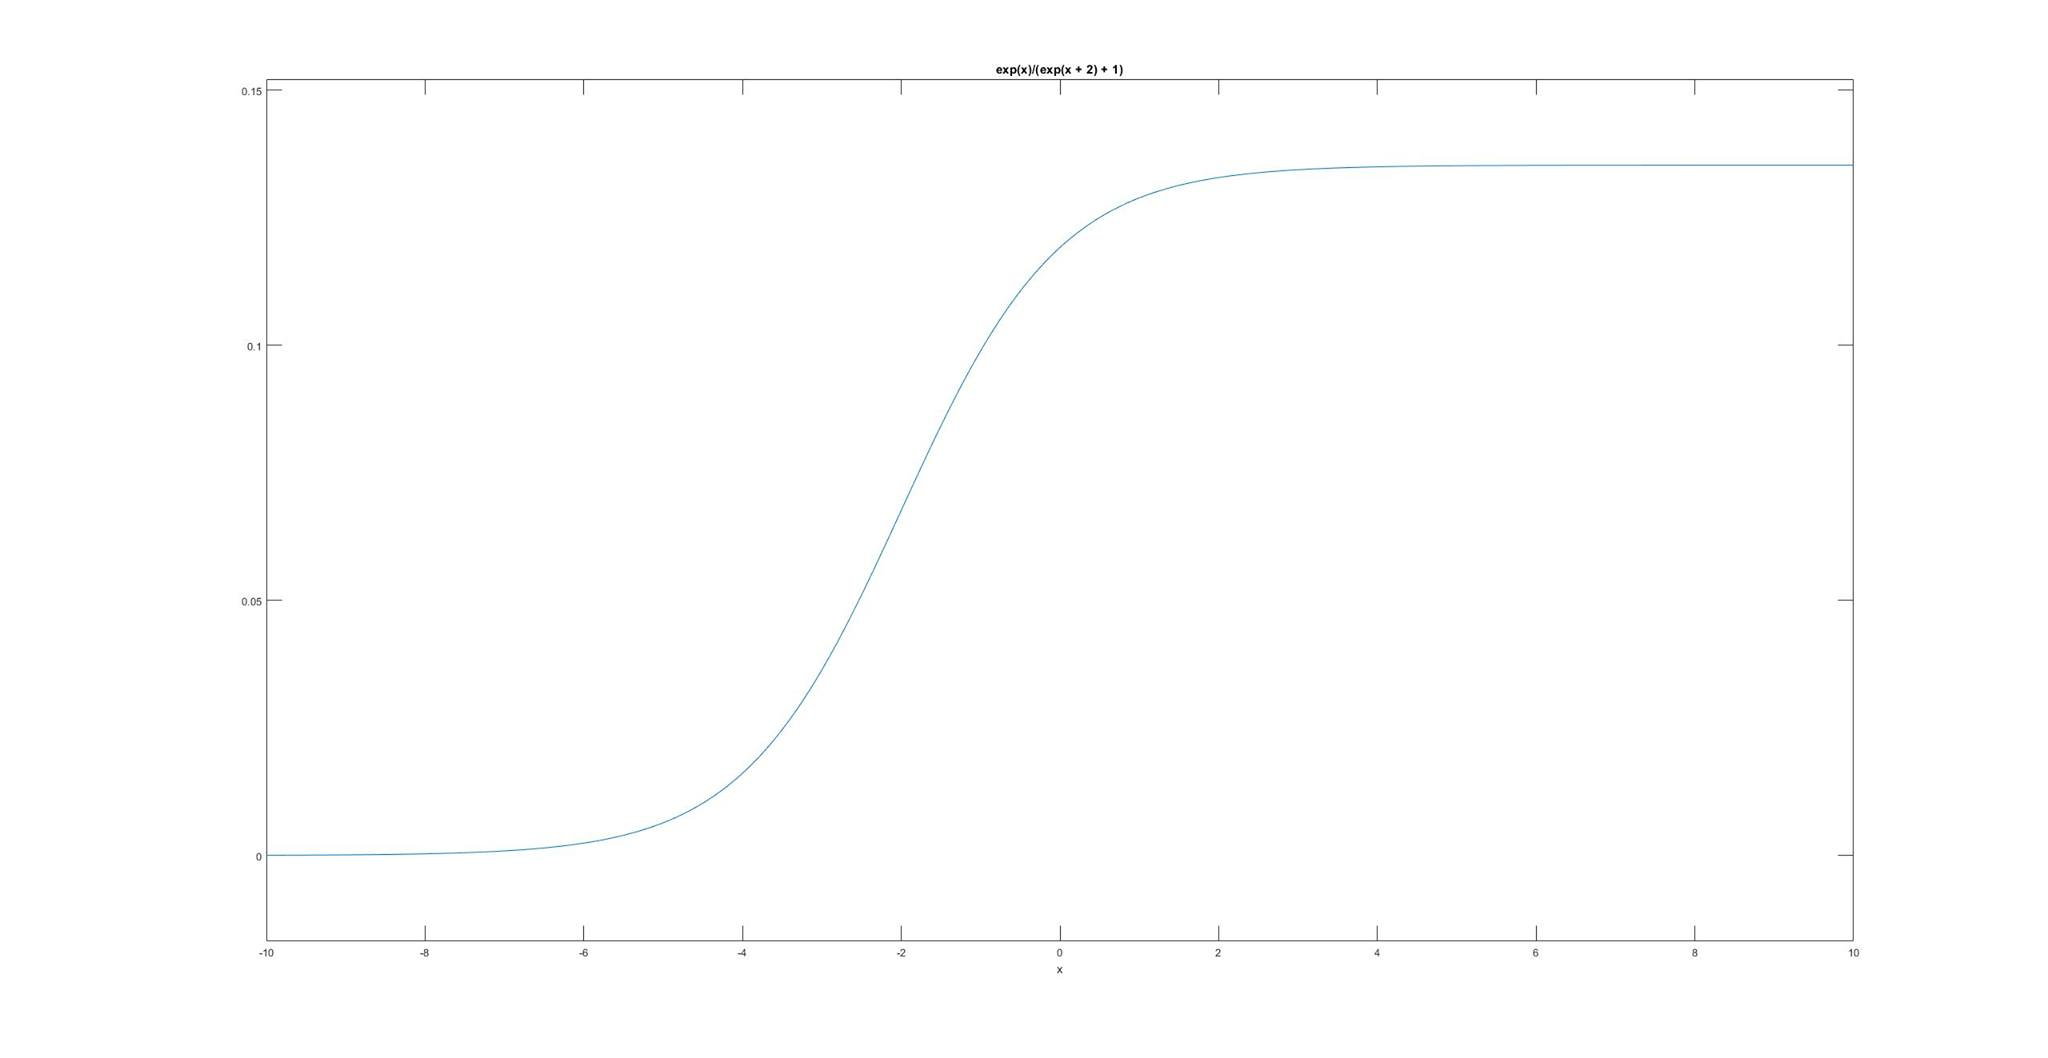
\includegraphics[width=0.8\textwidth]{beta_pos.jpg}
          \captionof{figure}{$\eta(x)$ with postive $\beta_0$}
        \end{center}
        \begin{center}
          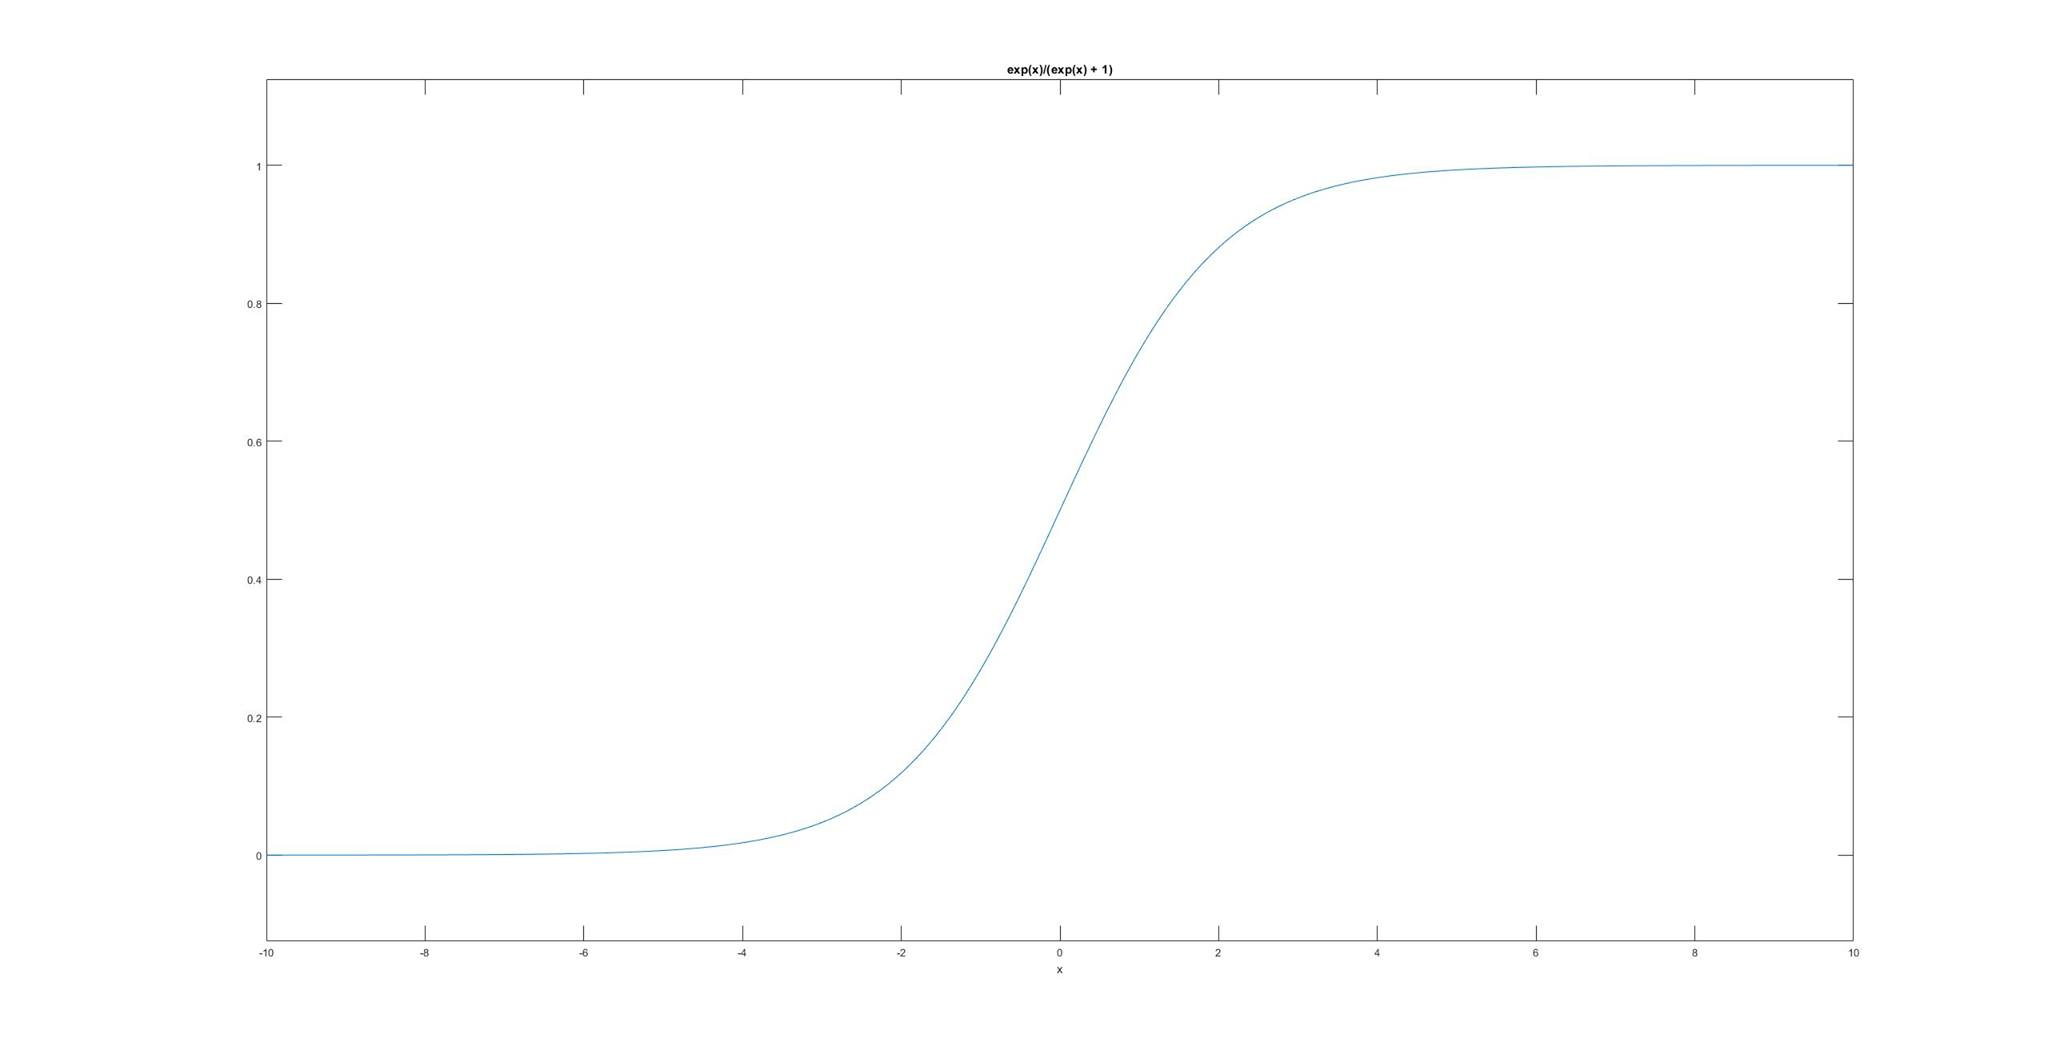
\includegraphics[width=0.8\textwidth]{beta_0.jpg}
          \captionof{figure}{$\eta(x)$ with $\beta_0 = 0$}
        \end{center}
        \begin{center}
          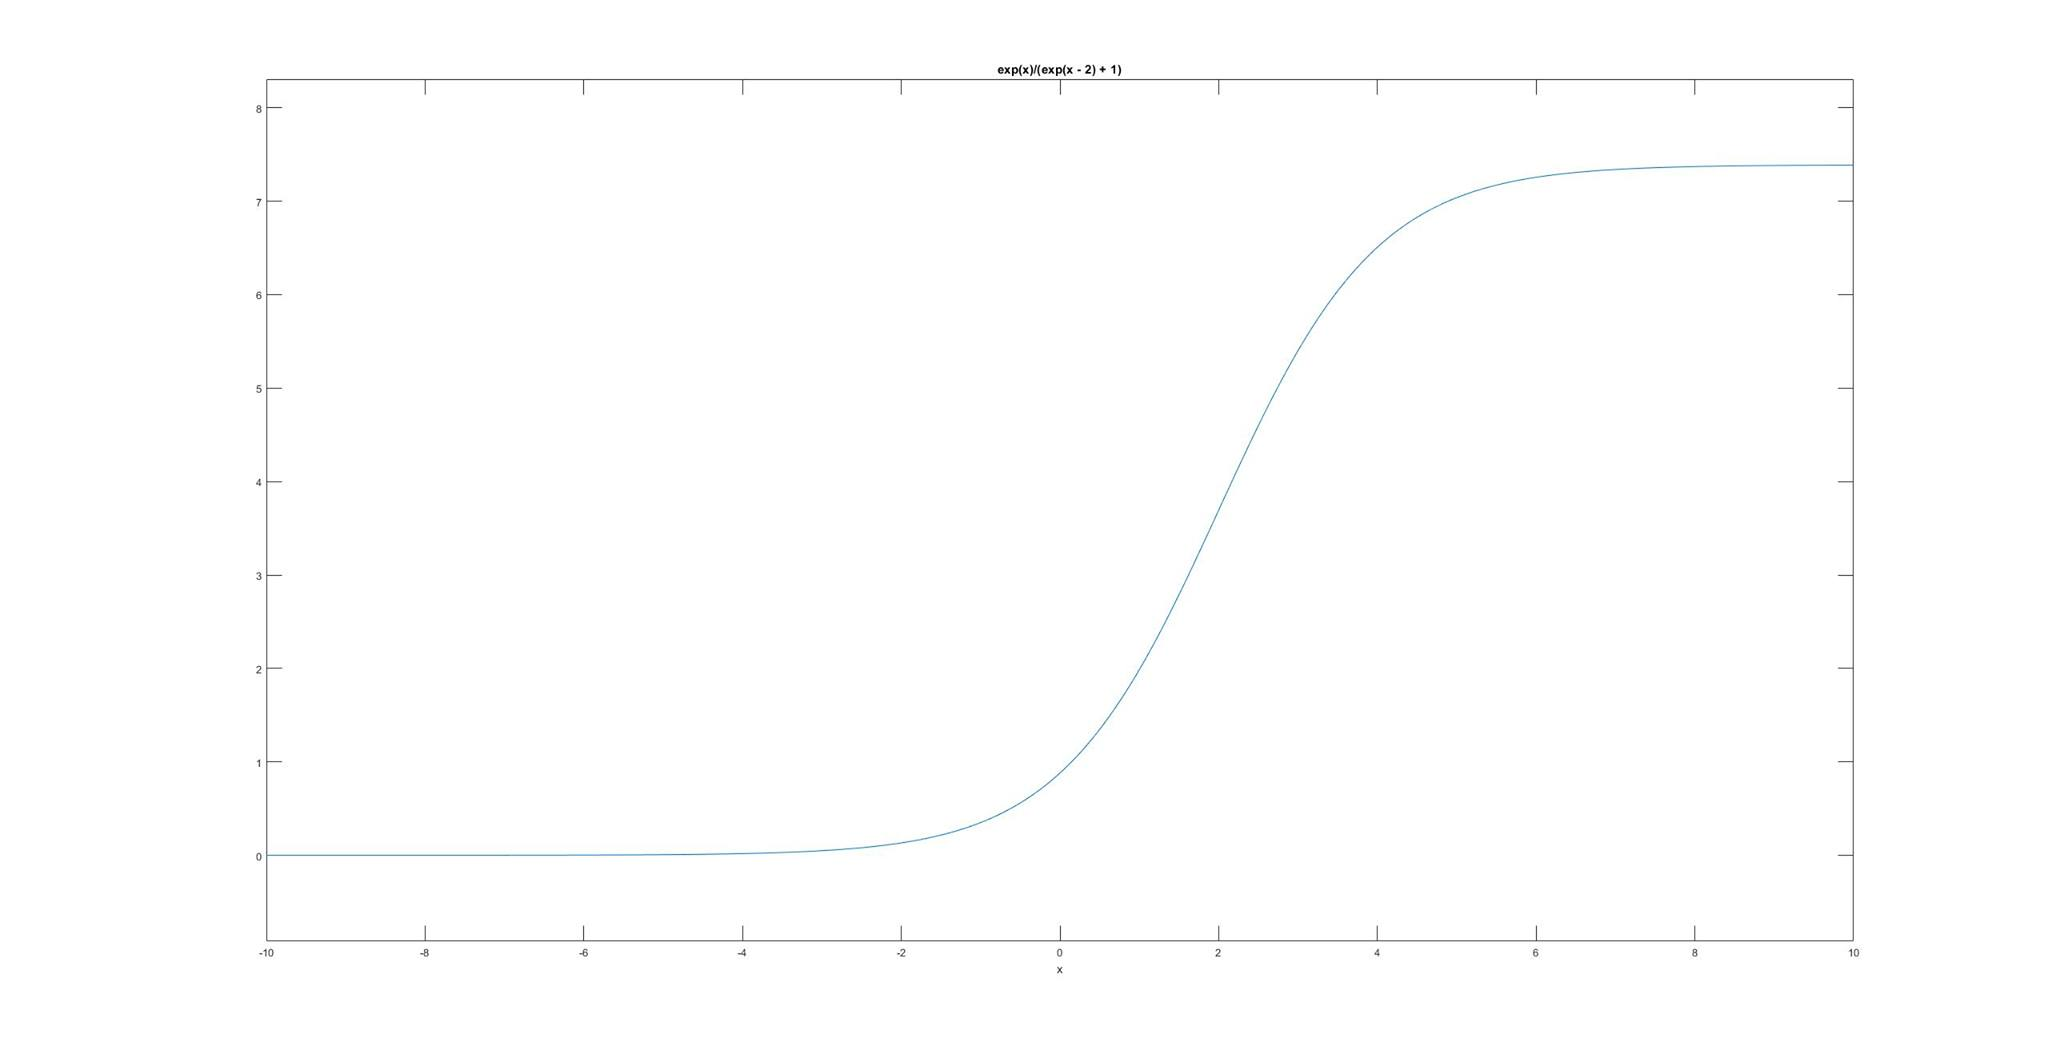
\includegraphics[width=0.8\textwidth]{beta_neg.jpg}
          \captionof{figure}{$\eta(x)$ with negative $\beta_0$}
        \end{center}

      \item We have that the likelihood is
        \begin{align*}
          \ell_{Y|X}(\beta) &= \log(\prod_{i=1}^n \mathbb{P}_\beta(Y_i|X_i)) \\
          &= \sum_{i=1}^n \log \left( \frac{1}{1+e^{\beta x_i}} \right) 1_{\{y_i = 0\}} + \log \left( \frac{e^{\beta x_i}}{1+e^{\beta x_i}} \right) 1_{\{y_i = 1\}}
        \end{align*}

      \item This simplifies the likelihood, we can rewrite the above as
        \begin{gather*}
          \ell_{Y|X}(\beta) = \sum_{x_i : x_i \leq 0} \log \left( \frac{1}{1+e^{\beta x_i}} \right) + \sum_{x_i : x_i > 0} \log \left( \frac{e^{\beta x_i}}{1+e^{\beta x_i}} \right)
        \end{gather*}
        Which both terms are bounded above by $\log(1)$. But, we have that as $\beta \rightarrow \infty$ that each term approaches $\log(1)$. Thus, $\hat{\beta}=\infty$.
    \end{enumerate}
  \end{enumerate}
\end{answer}

\clearpage
b
\begin{exercise}
  In this problem, we will show the linear discriminant analysis is equivalent to least square estimator. Suppose $\mathbb{P}(Y = 1) = p$, $\mathbb{P}(Y = -1) = 1 - p$, $X | Y = -1 \sim \mathcal{N}(\mu_1, \Sigma)$, and $X | Y = 1 \sim \mathcal{N}(\mu_2, \Sigma)$. Suppose we observe the samples $\mathcal{D}_1 = \{ Y_i, X_i \}_{i=1}^{n_1}$ for $Y_i = -1$ and $\mathcal{D}_2 = \{ Y_i, X_i \}_{i=1}^{n_2}$ for $Y_i = 1$.
  \begin{enumerate}[label=\arabic*)]
    \item Derive the Bayes classifier for this model. What is the maximum likelihood estimator of $p$, $\mu_1$, $\mu_2$, and $\Sigma$? Plug your MLE to the Bayes classifier and prove that it can be expressed as sign($\hat{w}^T x + \hat{b}$).

    \item Suppose we have two classes $\mathcal{D}_1 = \{ Y_i, X_i \}_{i=1}^{n_1}$ and $\mathcal{D}_2 = \{ Y_i, X_i \}_{i=1}^{n_2}$ . Let $n = n_1 + n_2$. We re-encode the two classes as $Y_i = -n/n_1$ if it belonds to $\mathcal{D}_1$ and $Y_i = n/n_2$ if it belonds to $\mathcal{D}_2$. Let $\hat{w}$ be the linear discriminant analysis solution you derived in Q4.1. Let the least square estimator be
      \begin{gather*}
        (\hat{\beta}_0, \hat{\beta}) = \argmin_{\beta_0, \beta} \sum_{i=1}^n (Y_i - \beta_0 - X_i^T \beta)^2
      \end{gather*}
      Prove that $\hat{\beta} \propto \hat{w}$.

    \item Construct a concrete binary class classification data sample \\ $\mathcal{D}_1 = \{ Y_i, X_i \}_{i=1}^{n_1}$ and $\mathcal{D}_2 = \{ Y_i, X_i \}_{i=1}^{n_2}$  in which the data from the two clases are linearly separable but the LDA does not separate the data. This implies that LDA is not always applicable.
  \end{enumerate}
\end{exercise}

\begin{answer}
  \leavevmode
  \begin{enumerate}[label=\arabic*)]
    \item We have
      \begin{gather*}
        \mathbb{P}(Y=1 | X=x) = \frac{p e^{-\frac{1}{2} (x - \mu_2)^T \Sigma^{-1} (x - \mu_2)}}{(1-p)e^{-\frac{1}{2} (x - \mu_1)^T \Sigma^{-1} (x - \mu_1)} + p e^{-\frac{1}{2} (x - \mu_2)^T \Sigma^{-1} (x - \mu_2)}}
      \end{gather*}
      We wish to find the condition with which $\mathbb{P}(Y = 1 | X=x) \geq \mathbb{P}(Y = -1 | X=x)$. That is
      \begin{align*}
        &\quad \mathbb{P}(Y = 1 | X=x) \geq \frac{1}{2} \\
        &\Longleftrightarrow 2p e^{-\frac{1}{2} (x - \mu_2)^T \Sigma^{-1} (x - \mu_2)} \\
        &\quad \quad \geq (1-p)e^{-\frac{1}{2} (x - \mu_1)^T \Sigma^{-1} (x - \mu_1)} + p e^{-\frac{1}{2} (x - \mu_2)^T \Sigma^{-1} (x - \mu_2)} \\
        &\Longleftrightarrow p e^{-\frac{1}{2} (x - \mu_2)^T \Sigma^{-1} (x - \mu_2)} \geq (1-p)e^{-\frac{1}{2} (x - \mu_1)^T \Sigma^{-1} (x - \mu_1)} \\
        &\Longleftrightarrow -\frac{1}{2} (x - \mu_2)^T \Sigma^{-1} (x - \mu_2) \geq \log \left( \frac{1-p}{p} \right) -\frac{1}{2} (x - \mu_1)^T \Sigma^{-1} (x - \mu_1) \\
        &\Longleftrightarrow 2(\mu_2 - \mu_1)^T \Sigma^{-1} x \geq 2 \log \left( \frac{1-p}{p} \right) + \mu_2^T \Sigma^{-1} \mu_2 - \mu_1^T \Sigma^{-1} \mu_1
      \end{align*}
      Thus, letting $w^T = 2(\mu_2 - \mu_1)^T \Sigma^{-1}$ and $b = -2\log \left( \frac{1-p}{p} \right) + \mu_2^T \Sigma^{-1} \mu_2 - \mu_1^T \Sigma^{-1} \mu_1$, we have that the Bayes classifier is
      \begin{gather*}
        h^*(x) = \text{sign}(w^T x + b)
      \end{gather*}
      Now for the MLE, we first write the log-likelihood
      \begin{gather*}
        \ell(Y,X) \propto - \sum_{i=1}^{n_1} \frac{1}{2} ((x_i - \mu_1)^T \Sigma^{-1}(x_i - \mu_1) + \log \lvert \Sigma \rvert) + \sum_{i=1}^{n_1} \log (1-p) \\
        - \sum_{i=1}^{n_2} \frac{1}{2} ((x_i - \mu_2)^T \Sigma^{-1}(x_i - \mu_2) + \log \lvert \Sigma \rvert) + \sum_{i=1}^{n_2} \log (p)
      \end{gather*}
      Thus, the MLE for $p$ is:
      \begin{gather*}
        \frac{\partial \ell}{\partial p} = -n_1 \frac{1}{1-\hat{p}} - \frac{n_2}{\hat{p}} = 0 \\
        \implies \hat{p} = \frac{n_2}{n_1 + n_2}
      \end{gather*}
      The MLE for $\mu_i$:
      \begin{gather*}
        \nabla_{\mu_i} \ell = \sum_{i=1}^{n_i} \hat{\Sigma}^{-1} (x_i - \hat{\mu}_i) = 0 \\
        \implies \hat{\mu}_i = \frac{1}{n_i} \sum_{i=1}^{n_i} x_i
      \end{gather*}
      Finally, the MLE for $\Sigma$, we take the matrix derivative:
      \begin{align*}
        (D_\Sigma \ell)(\Delta \Sigma) = \sum_{i=1}^{n_1} (x_i - \hat{\mu_1})^T \hat{\Sigma}^{-1} \Delta \Sigma \hat{\Sigma}^{-1} (x_i - \hat{\mu_1}) - n_1 \text{trace}(\hat{\Sigma}^{-1} \Delta \Sigma) \\
        + \sum_{i=1}^{n_2} (x_i - \hat{\mu_2})^T \hat{\Sigma}^{-1} \Delta \Sigma \hat{\Sigma}^{-1} (x_i - \hat{\mu_2}) - n_2 \text{trace}(\hat{\Sigma}^{-1} \Delta \Sigma) = 0
      \end{align*}
      After some algebra
      \begin{gather*}
        \hat{\Sigma} = \frac{1}{n_1 + n_2} \left( \sum_{i=1}^{n_1} (x_i - \hat{\mu_1})(x_i - \hat{\mu_1})^T + \sum_{i=1}^{n_2} (x_i - \hat{\mu_2})(x_i - \hat{\mu_2})^T \right)
      \end{gather*}
      Thus, using our $w$ and $b$ from before, define
      \begin{gather*}
        \hat{w} = 2(\hat{\mu}_2 - \hat{\mu}_1)^T \hat{\Sigma}^{-1} \\
        \hat{b} = -2\log \left( \frac{1-\hat{p}}{\hat{p}} \right) + \hat{\mu_2}^T \hat{\Sigma}^{-1} \hat{\mu_2} - \hat{\mu_1}^T \hat{\Sigma}^{-1} \hat{\mu_1}
      \end{gather*}
      So we have $h^*(x) = \text{sign} (\hat{w}^T x + \hat{b})$.

    \item As usual, we expand out the quadratic term of the LSE
      \begin{gather*}
        f = \sum_{i=1}^n (Y_i - \beta_0 - X_i^T \beta)^2 \\
        = \sum_{i=1}^n Y_i^2 + \beta_0^2 + (X_i^T \beta)^2 - 2 Y_i \beta_0 - 2Y_i X_i^T \beta + 2 \beta_0 X_i^T \beta
      \end{gather*}
      Now we take the derivatives and set them to 0
      \begin{align*}
        \frac{\partial f}{\partial \beta_0} = 2 n \beta_0 - 2 \sum_{i=1}^n Y_i + 2 \sum_{i=1}^n X_i^T \beta
      \end{align*}
      By re-encoding the $Y_i$'s, the sum in the above function is 0. Thus
      \begin{gather*}
        \hat{\beta}_0 = -\frac{1}{n} \sum_{i=1}^n X_i^T \beta
      \end{gather*}
      Now for $\beta$, we have
      \begin{gather*}
        \nabla_\beta f = 2 \sum_{i=1}^n (X_i \beta) X_i - 2 \sum_{i=1}^n Y_i X_i + 2 \beta_0 \sum_{i=1}^n X_i = 0
      \end{gather*}
      Now, note that $\sum_{i=1}^n Y_i X_i = (\hat{\mu}_2 - \hat{\mu}_1)n$. Also, plugging in our solution for $\beta_0$ results in
      \begin{gather*}
        \sum_{i=1}^n (X_i X_i^T) \beta = (\hat{\mu}_2 - \hat{\mu}_1)n + \frac{1}{n} \left( \sum_{i=1}^n X_i^T \right) \left( \sum_{i=1}^n X_i \right) \beta
      \end{gather*}
      So we conclude that $\hat{\beta} = \hat{\Sigma}^{-1} (\hat{\mu}_2 - \hat{\mu}_1)$ which is exactly the definition of $\hat{w}$ without the 2. Thus, $\hat{\beta} \propto \hat{w}$.

    \item The trick for this is to pick one set that is clustered together and then one element from the other that is close to the other set. For example, let us consider the 1 dimensional example:
      \begin{gather*}
        \mathcal{D}_1 = \{ (-1,0), (-1,0) \} \\
        \mathcal{D}_2= \{ (1,1), (1,11) \}
      \end{gather*}
      This is clearly separable, 0.5 separates all the $x_i$. Now, we compute the MLE's
      \begin{gather*}
        \hat{p} = 1/2 \\
        \hat{\mu}_1 = 0 \\
        \hat{\mu}_2 = 6 \\
        \hat{\Sigma} = \frac{1}{4} (0^2 + 0^2 + (1-6)^2 + (11-6)^2) = 12.5
      \end{gather*}
      Thus, using what we derived in 4.1
      \begin{gather*}
        \hat{w} = 2 (6 - 0)/12.5 = 0.96 \\
        \hat{b} = - 2 \log(1) + 0^2 / 12.5 - 6^2 /12.5 = -2.88
      \end{gather*}
      Which means $h^*(x) = \text{sign}(0.96 x - 2.88)$. Now we take $(1,1)$ which is in $\mathcal{D}_2$ and we get
      \begin{gather*}
        h^*(1) = \text{sign}(0.96 - 2.88) = -1
      \end{gather*}
      Which is wrongly classified as $\mathcal{D}_1$.
  \end{enumerate}
\end{answer}

\clearpage

\begin{exercise}
  Let $\mathcal{D} = \{ (y_i, x_i) \}_{i=1}^n$ be the classification dataset, where $y_i = \{ +1, -1\}$. We say a linear separator $w$ ($\lVert w \rVert = 1$) for $\mathcal{D}$ has margin $\gamma$ if $y_i \cdot (w^T x_i) > \gamma$ for all $1 \leq i \leq n$. If there exists such a separator, we say $\mathcal{D}$ is separable by a margin of $\gamma$. We know that SVM is an algorithm to maximize the margin. In this problem, we will explore the limit of SVM by deriving the relations between the margin and the linear classifier.
  \begin{enumerate}[label=\arabic*)]
    \item This problem shows the lower bound of samples we need to have reasonable classification error. We consider the unit ball $\mathcal{X} = \{ x \in \mathbb{R}^d : \lVert x \rVert_2 = 1 \}$. Show that there exists two disjoint sets $\mathcal{D}_0, \mathcal{D}_1 \subseteq \mathcal{X}$ with margin $\gamma$, where $1/\gamma^2 \leq d$ such that given any $s$ samples from $\mathcal{D}_0$ and $s$ samples from $\mathcal{D}_1$, where $s = 1/(100 \gamma^2)$, there exists a unit vector $w$ satisfying:
      \begin{enumerate}[label=\arabic*)]
        \item The vector $w$ separates the $2s$ samples by a margin $\gamma$;
        \item But $w$ misclassifies at least 1/3 of the points in $\mathcal{D}_0$ and $\mathcal{D}_1$.
      \end{enumerate}
      (\textbf{Hint:} You may prove this by constructing $x_i$'s with margin $\gamma$ for any possible labels of $y_i$'s. Therefore you can construct a $w$ separating any training data but it misclassifies the remaining data.)

    \item This problem show that the margin may decrease exponentially with the dimension of the dataset on the cube $\{0,1\}^d \backslash \{0\}$. Suppose we have points $x \in \{0,1\}^d$ and we label $x$ as +1 if and only if the least $i$ for which $x_i = 1$ is odd. Otherwise, we label $x$ as -1. Show that we can separate these two classes by a linear separator:
      \begin{gather*}
        \sum_{i=1}^d \frac{(-1)^{i-1} x_i}{2^{i-1}} > 0
      \end{gather*}
      Prove that we cannot have a linear separator for the above dataset with margin at least $1/f(d)$ where $f(d)$ is bounded above by a polynomial function of $d$.
  \end{enumerate}
\end{exercise}

\begin{answer}
  \leavevmode
  \begin{enumerate}[label=\arabic*)]
    \item Let us consider the sets $\mathcal{D}_0 = \{e_i\}_{i=1}^{d/2} \in \mathcal{X}$ and $\mathcal{D}_1 = \{e_i\}_{i=d/2}^{d} \in \mathcal{X}$, where $e_i$ is the canonical basis vector. Then we have $s = 1/(100 \gamma^2) \leq d/100$ and so we have sufficient samples to draw from. Label all the points in $\mathcal{D}_0$ with 1 and all the points in $\mathcal{D}_1$ with +1. Now we define $w$ as follows
      \begin{gather*}
        w_i = \begin{cases}
          0 & \text{ if } e_i \notin \mathcal{D}_0 \cup \mathcal{D}_1 \\
          \frac{1}{\sqrt{2s}} & \text{ if } e_i \notin \mathcal{D}_0 \\
          -\frac{1}{\sqrt{2s}} & \text{ if } e_i \notin \mathcal{D}_0
        \end{cases}
      \end{gather*}
      By construction, we have that $w^T x_i = y_i w^T x_i = \frac{1}{\sqrt{2s}} > \gamma$. Thus, $\mathcal{D}_0$ and $\mathcal{D}_1$ are seprable by $\gamma$. Now, we swap 1/3 of the elements in $\mathcal{D}_0$ with 1/3 of the elements in $\mathcal{D}_1$. This is still separable by the equivalent $w$ defined above but misclassifies 1/3 of the points.

    \item $x_i$ denotes the first entry that is not 0. Now suppose $y_i = 1$. That is, $i$ is odd. Then
      \begin{gather*}
        y_i \sum_{j=1}^d \frac{(-1)^{j-1}}{2^{j-1}}x_j = \sum_{j=i+1}^d \frac{(-1)^{j-1}}{2^{j-1}}x_j + \frac{1}{2^{i-1}}
      \end{gather*}
      But this is strictly positive as
      \begin{gather*}
        \lvert \sum_{j=i+1}^d \frac{(-1)^{j-1}}{2^{j-1}}x_j \rvert < \frac{1}{2^{i-1}}
      \end{gather*}
      Likewise, if we take $y_i = -1$, then $i$ is even
      \begin{gather*}
        y_i \sum_{j=1}^d \frac{(-1)^{j-1}}{2^{j-1}}x_j = \sum_{j=i+1}^d \frac{(-1)^{j}}{2^{j-1}}x_j + \frac{1}{2^{i-1}} \\
        \text{and } \lvert \sum_{j=i+1}^d \frac{(-1)^{j}}{2^{j-1}}x_j \rvert < \frac{1}{2^{i-1}}
      \end{gather*}
      Therefore, by picking $w_i = \frac{(-1)^{i-1}}{2^{i-1}}$, $w$ separates the data.

      Now, we consider a separating $w$ with $\lVert w \rVert = 1$ that separates the dataset with margin $\gamma$. Again, take $x_i = e_i$. Then, by definition we have
      \begin{gather*}
       y_i e_i^T w = (-1)^i w_i > \gamma
      \end{gather*}
      Which implies that $\lVert w \rVert_1 > d \gamma$ (by taking for any $i \in \{1, \mathellipsis, d\}$). But, we also have
      \begin{gather*}
        \lVert w \rVert_1 \leq \sqrt{d} \lvert w \rVert_2 = \sqrt{d} \\
        \implies \gamma < \frac{1}{\sqrt{d}}
      \end{gather*}
      But $\sqrt{d}$ is smaller than any polynomial, thus we have the shown the result
  \end{enumerate}
\end{answer}

\end{document}